%
% File acl2021.tex
%
%% Based on the style files for EMNLP 2020, which were
%% Based on the style files for ACL 2020, which were
%% Based on the style files for ACL 2018, NAACL 2018/19, which were
%% Based on the style files for ACL-2015, with some improvements
%%  taken from the NAACL-2016 style
%% Based on the style files for ACL-2014, which were, in turn,
%% based on ACL-2013, ACL-2012, ACL-2011, ACL-2010, ACL-IJCNLP-2009,
%% EACL-2009, IJCNLP-2008...
%% Based on the style files for EACL 2006 by 
%%e.agirre@ehu.es or Sergi.Balari@uab.es
%% and that of ACL 08 by Joakim Nivre and Noah Smith

\documentclass[11pt,a4paper]{article}
\usepackage[hyperref]{acl2021}
\usepackage{times}
\usepackage{listings}
\usepackage{latexsym}
\usepackage{graphicx}
\graphicspath{ {./images/} }
\renewcommand{\UrlFont}{\ttfamily\small}
\lstset {
  basicstyle=\itshape,
  xleftmargin=3em,
  literate={->}{$\rightarrow$}{2}
           {α}{$\alpha$}{1}
           {δ}{$\delta$}{1}
}
% This is not strictly necessary, and may be commented out,
% but it will improve the layout of the manuscript,
% and will typically save some space.
\usepackage{microtype}

%\aclfinalcopy % Uncomment this line for the final submission
%\def\aclpaperid{***} %  Enter the acl Paper ID here

%\setlength\titlebox{5cm}
% You can expand the titlebox if you need extra space
% to show all the authors. Please do not make the titlebox
% smaller than 5cm (the original size); we will check this
% in the camera-ready version and ask you to change it back.

\newcommand\BibTeX{B\textsc{ib}\TeX}

\title{UWRT Semantic Parser Assistant}

\author{Jake Imyak \\
  Affiliation / Address line 1 \\
  Affiliation / Address line 2 \\
  Affiliation / Address line 3 \\
  \texttt{imyak.1@osu.edu} \\\And
  Second Author \\
  Affiliation / Address line 1 \\
  Affiliation / Address line 2 \\
  Affiliation / Address line 3 \\
  \texttt{email@domain} \\}

\date{December 10th, 2021}

\begin{document}
\maketitle
\begin{abstract}
This document contains the instructions for preparing a manuscript for the proceedings of ACL-IJCNLP 2021.
The document itself conforms to its own specifications, and is therefore an example of what your manuscript should look like.
These instructions should be used for both papers submitted for review and for final versions of accepted papers.
Authors are asked to conform to all the directions reported in this document.
\end{abstract}

\section{Credits}

This document has been adapted by Roberto Navigli
from the instructions for earlier ACL, NAACL and EMNLP proceedings, including those for 
EMNLP 2020 by Yulan He,
ACL 2020 by Steven Bethard, Ryan Cotterrell and Rui Yan, 
ACL 2019 by Douwe Kiela and Ivan Vuli\'{c},
NAACL 2019 by Stephanie Lukin and Alla Roskovskaya, 
ACL 2018 by Shay Cohen, Kevin Gimpel, and Wei Lu, 
NAACL 2018 by Margaret Michell and Stephanie Lukin,
2017/2018 (NA)ACL bibtex suggestions from Jason Eisner,
ACL 2017 by Dan Gildea and Min-Yen Kan, 
NAACL 2017 by Margaret Mitchell, 
ACL 2012 by Maggie Li and Michael White, 
ACL 2010 by Jing-Shing Chang and Philipp Koehn, 
ACL 2008 by Johanna D. Moore, Simone Teufel, James Allan, and Sadaoki Furui, 
ACL 2005 by Hwee Tou Ng and Kemal Oflazer, 
ACL 2002 by Eugene Charniak and Dekang Lin, 
and earlier ACL and EACL formats written by several people, including
John Chen, Henry S. Thompson and Donald Walker.
Additional elements were taken from the formatting instructions of the \emph{International Joint Conference on Artificial Intelligence} and the \emph{Conference on Computer Vision and Pattern Recognition}.

\section{Introduction}

The following instructions are directed to authors of papers submitted to ACL-IJCNLP 2021 or accepted for publication in its proceedings.
All authors are required to adhere to these specifications.
Authors are required to provide a Portable Document Format (PDF) version of their papers.
\textbf{The proceedings are designed for printing on A4 paper.}


\section{Data}

A dataset was to be created in order to use natural language utterances to lambda calculus expressions that a parser would be able to recognize to convert to a finite state machine. For reference, the following datasets were considered: the Geoquery set (Zettlemoyer and Collins, 2005) and General Purpose Service Robotics commands set (Walker, Peng, and Cakmak, 2019). The Geoquery dataset provided a foundation for a grammar to follow for the lambda calculus expression such that consistency would hold for our parser. Moreover, the gpsr dataset provided an ample amount of examples and different general purpose robotics commands that could be extended within the dataset we curated. 

The dataset followed the following form: natural language utterance followed by a tab then a lambda calculus expression. The lambda calculus expression is of the form ( seq ( action0 ( \$0 ( parameter ) ) ) ... ( actionN ( \$N ( parameter ) ) ). The power of the following expression is that it can be extended to N number of actions in a given sequence, meaning that a user can hypothetically type in a very complex string of action and an expression will be constructed for said sequence. Moreover, the format of our dataset allows for it to be extended for any type of robotics command that a user may have. They just need to include examples in the train set with said action and the model will consider it.

\noindent The formal grammar is:

\noindent $<seq> -> ( seq ( action ) [ (action) ] )$

\noindent $<action> -> actionName [ (parameter ] )$

\noindent $<$parameter$>$ - $>$ PARAM\_NAME \lambda ( \$n ( n ) )

The dataset we created had 1000 entries in the training dataset and 250 entries in the test dataset. The size of the vocabulary $|V|=N$, which is similar in vocabulary size to the GeoQuery dataset. The expressions currently increase in complexity in terms of the number of actions within the sequence. A way to extend the complexity of the expressions would make the $<seq>$ tag a nonterminal to chain together nested sequences. 

\section{Model}
\label{sec:length}

\subsection{Seq2Seq Model}
We decided to use the model presented in "Language to Logical Form with Neural Attention" (Dong and Lapata, 2016). There was an implementation on GitHub (add footnote) utilizing Google's Tensorflow library to handle all implementation details of the following model. The part of the paper that was presented was the Sequence to Sequence model with an attention mechanism.  

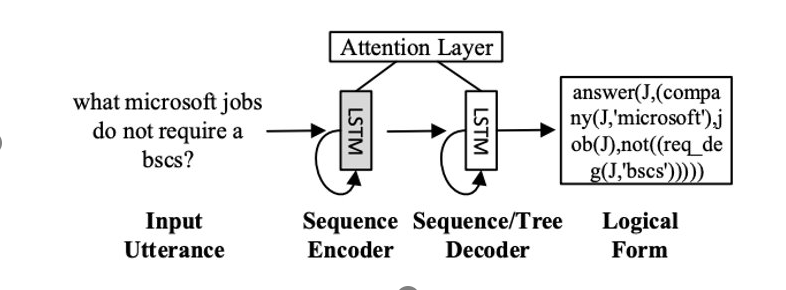
\includegraphics[scale=.5]{figure1}
\noindent Figure 1: Process of how input natural language are encoded and decoded via recurrent neural networks and an attention mechanism to find the utterance's respective natural language form. (Dong and Lapata, 2016)

The model interprets both the input and output from the network as sequences of information. This process is represented in Figure 1: input is passed to the encoder, then passed through the decoder, and through using the attention mechanism, we can get an output that is a lambda calculus expression. Both of these sequences can be represented as L-layer recurrent neural networks with long short-term memory (LSTM) that are used to take the tokens from the sentences and the expressions we have. The model creates 200 (can be changed to increase and decrease the size of the network) units of both LSTM cells and GRU cells. The GRU cells are used to help compensate for the vanishing gradient problem. These LSTM and GRU cells are used in the input sequence to encode $x_1, ..., x_{q}$ into vectors. Then these vectors are what form the hidden state of the beginning of the sequence in the decoder. Then in the decoder, the topmost LSTM cell predicts the t-th output token by taking the softmax of the parameter matrix and the vector from the LSTM cell multiplied by a one-hot vector used to compute the probability of the output from the probability distribution. The softmax used here is sampled softmax, which only takes into account a subset of our vocabulary V rather than everything to help alleviate the difficulty of finding the softmax of a large vocabulary. 

\subsection{Attention Mechanism}
The model also implemented an attention mechanism to help with the predicted values. The motivation behind the attention mechanism is to use the input sequence in the decoding process since it is relevant information for the prediction of the output token. To achieve this, a context vector is created which is the weighted sums of the hidden vectors in the encoder. Then this context vector is used as context to find the probability of generating a given output. 

\subsection{Training}
To train the model, the objective is the maximize the likelihood of predicting the correct logical form given some natural language expression. Hence, the goal is to minimize the sum of the log probability of predicting logical form a given natural language utterance q summed over all training pairs. The model used the RMSProp algorithm which is an extension of the Adagrad optimizer but utilizes learning rate adaptation. Dropout is also used for regularization which helps out with a smaller datasets to prevent overfitting.

\subsection{Inference}
To perform inference, the argmax is found of the probability of candidate output given the natural language utterance. Since it is not possible to find the probability of all possible outputs, the probability is put in a form such that a beam search can be employed to generate each individual token of lambda calculus expression to get the appropriate output. 

\section{Results}
As reviewing will be double-blind, papers submitted for review should not include any author information (such as names or affiliations). Furthermore, self-references that reveal the author's identity, \emph{e.g.},
\begin{quote}
We previously showed \citep{Gusfield:97} \ldots
\end{quote}
should be avoided. Instead, use citations such as 
\begin{quote}
\citet{Gusfield:97} previously showed\ldots
\end{quote}
Please do not use anonymous citations and do not include acknowledgements.
\textbf{Papers that do not conform to these requirements may be rejected without review.}

Any preliminary non-archival versions of submitted papers should be listed in the submission form but not in the review version of the paper.
Reviewers are generally aware that authors may present preliminary versions of their work in other venues, but will not be provided the list of previous presentations from the submission form. 

Please do not include github links that reveal the authors' identities in your submission. If you feel it is important to include your source code, you can zip the code and submit it to softconf. 

Once a paper has been accepted to the conference, the camera-ready version of the paper should include the author's names and affiliations, and is allowed to use self-references and provide the related github link.


\paragraph{\LaTeX-specific details:}
For an anonymized submission, ensure that {\small\verb|\aclfinalcopy|} at the top of this document is commented out, and that you have filled in the paper ID number (assigned during the submission process on softconf) where {\small\verb|***|} appears in the {\small\verb|\def\aclpaperid{***}|} definition at the top of this document.
For a camera-ready submission, ensure that {\small\verb|\aclfinalcopy|} at the top of this document is not commented out.


\section{Multiple Submission Policy}

ACL-IJCNLP 2021 will not consider any paper that is under review in a journal or another conference at the time of submission, and submitted papers must not be submitted elsewhere during the ACL-IJCNLP 2021 review period. This policy covers all refereed and archival conferences and workshops (e.g., NAACL). The only exception is that a paper can be dual-submitted to both ACL-IJCNLP 2021 and an ACL-IJCNLP workshop. 

In addition, we will not consider any paper that overlaps significantly in content or results with papers that will be (or have been) published elsewhere. 
Authors submitting more than one paper to ACL-IJCNLP 2021 must ensure that their submissions do not overlap significantly ($>25$\%) with each other in content or results.

\section{Formatting Instructions}

Manuscripts must be in two-column format.
Exceptions to the two-column format include the title, authors' names and complete addresses, which must be centered at the top of the first page, and any full-width figures or tables (see the guidelines in Section~\ref{ssec:title-authors}).
\textbf{Type single-spaced.}
Start all pages directly under the top margin.
The manuscript should be printed single-sided and its length should not exceed the maximum page limit described in Section~\ref{sec:length}.
Pages should be numbered in the version submitted for review, but \textbf{pages should not be numbered in the camera-ready version}.

\paragraph{\LaTeX-specific details:}
The style files will generate page numbers when {\small\verb|\aclfinalcopy|} is commented out, and remove them otherwise.


\subsection{File Format}
\label{sect:pdf}

For the production of the electronic manuscript you must use Adobe's Portable Document Format (PDF).
Please make sure that your PDF file includes all the necessary fonts (especially tree diagrams, symbols, and fonts with Asian characters).
When you print or create the PDF file, there is usually an option in your printer setup to include none, all or just non-standard fonts.
Please make sure that you select the option of including ALL the fonts.
\textbf{Before sending it, test your PDF by printing it from a computer different from the one where it was created.}
Moreover, some word processors may generate very large PDF files, where each page is rendered as an image.
Such images may reproduce poorly.
In this case, try alternative ways to obtain the PDF.
One way on some systems is to install a driver for a postscript printer, send your document to the printer specifying ``Output to a file'', then convert the file to PDF.

It is of utmost importance to specify the \textbf{A4 format} (21 cm x 29.7 cm) when formatting the paper.
Print-outs of the PDF file on A4 paper should be identical to the hardcopy version.
If you cannot meet the above requirements about the production of your electronic submission, please contact the publication chairs as soon as possible.

\paragraph{\LaTeX-specific details:}
PDF files are usually produced from \LaTeX{} using the \texttt{\small pdflatex} command.
If your version of \LaTeX{} produces Postscript files, \texttt{\small ps2pdf} or \texttt{\small dvipdf} can convert these to PDF.
To ensure A4 format in \LaTeX, use the command {\small\verb|\special{papersize=210mm,297mm}|}
in the \LaTeX{} preamble (below the {\small\verb|\usepackage|} commands) and use \texttt{\small dvipdf} and/or \texttt{\small pdflatex}; or specify \texttt{\small -t a4} when working with \texttt{\small dvips}.

\subsection{Layout}
\label{ssec:layout}

Format manuscripts two columns to a page, in the manner these
instructions are formatted.
The exact dimensions for a page on A4 paper are:

\begin{itemize}
\item Left and right margins: 2.5 cm
\item Top margin: 2.5 cm
\item Bottom margin: 2.5 cm
\item Column width: 7.7 cm
\item Column height: 24.7 cm
\item Gap between columns: 0.6 cm
\end{itemize}

\noindent Papers should not be submitted on any other paper size.
If you cannot meet the above requirements about the production of your electronic submission, please contact the publication chairs above as soon as possible.

\subsection{Fonts}

For reasons of uniformity, Adobe's \textbf{Times Roman} font should be used.
If Times Roman is unavailable, you may use Times New Roman or \textbf{Computer Modern Roman}.

Table~\ref{font-table} specifies what font sizes and styles must be used for each type of text in the manuscript.

\begin{table}
\centering
\begin{tabular}{lrl}
\hline \textbf{Type of Text} & \textbf{Font Size} & \textbf{Style} \\ \hline
paper title & 15 pt & bold \\
author names & 12 pt & bold \\
author affiliation & 12 pt & \\
the word ``Abstract'' & 12 pt & bold \\
section titles & 12 pt & bold \\
subsection titles & 11 pt & bold \\
document text & 11 pt  &\\
captions & 10 pt & \\
abstract text & 10 pt & \\
bibliography & 10 pt & \\
footnotes & 9 pt & \\
\hline
\end{tabular}
\caption{\label{font-table} Font guide. }
\end{table}

\paragraph{\LaTeX-specific details:}
To use Times Roman in \LaTeX2e{}, put the following in the preamble:
\begin{quote}
\small
\begin{verbatim}
\usepackage{times}
\usepackage{latexsym}
\end{verbatim}
\end{quote}


\subsection{Ruler}
A printed ruler (line numbers in the left and right margins of the article) should be presented in the version submitted for review, so that reviewers may comment on particular lines in the paper without circumlocution.
The presence or absence of the ruler should not change the appearance of any other content on the page.
The camera ready copy should not contain a ruler.

\paragraph{Reviewers:}
note that the ruler measurements may not align well with lines in the paper -- this turns out to be very difficult to do well when the paper contains many figures and equations, and, when done, looks ugly.
In most cases one would expect that the approximate location will be adequate, although you can also use fractional references (\emph{e.g.}, this line ends at mark $295.5$).

\paragraph{\LaTeX-specific details:}
The style files will generate the ruler when {\small\verb|\aclfinalcopy|} is commented out, and remove it otherwise.

\subsection{Title and Authors}
\label{ssec:title-authors}

Center the title, author's name(s) and affiliation(s) across both columns.
Do not use footnotes for affiliations.
Place the title centered at the top of the first page, in a 15-point bold font.
Long titles should be typed on two lines without a blank line intervening.
Put the title 2.5 cm from the top of the page, followed by a blank line, then the author's names(s), and the affiliation on the following line.
Do not use only initials for given names (middle initials are allowed).
Do not format surnames in all capitals (\emph{e.g.}, use ``Mitchell'' not ``MITCHELL'').
Do not format title and section headings in all capitals except for proper names (such as ``BLEU'') that are
conventionally in all capitals.
The affiliation should contain the author's complete address, and if possible, an electronic mail address.

The title, author names and addresses should be completely identical to those entered to the electronical paper submission website in order to maintain the consistency of author information among all publications of the conference.
If they are different, the publication chairs may resolve the difference without consulting with you; so it is in your own interest to double-check that the information is consistent.

Start the body of the first page 7.5 cm from the top of the page.
\textbf{Even in the anonymous version of the paper, you should maintain space for names and addresses so that they will fit in the final (accepted) version.}


\subsection{Abstract}
Use two-column format when you begin the abstract.
Type the abstract at the beginning of the first column.
The width of the abstract text should be smaller than the
width of the columns for the text in the body of the paper by 0.6 cm on each side.
Center the word \textbf{Abstract} in a 12 point bold font above the body of the abstract.
The abstract should be a concise summary of the general thesis and conclusions of the paper.
It should be no longer than 200 words.
The abstract text should be in 10 point font.

\subsection{Text}
Begin typing the main body of the text immediately after the abstract, observing the two-column format as shown in the present document.

Indent 0.4 cm when starting a new paragraph.

\subsection{Sections}

Format section and subsection headings in the style shown on the present document.
Use numbered sections (Arabic numerals) to facilitate cross references.
Number subsections with the section number and the subsection number separated by a dot, in Arabic numerals.

\subsection{Footnotes}
Put footnotes at the bottom of the page and use 9 point font.
They may be numbered or referred to by asterisks or other symbols.\footnote{This is how a footnote should appear.}
Footnotes should be separated from the text by a line.\footnote{Note the line separating the footnotes from the text.}

\subsection{Graphics}

Place figures, tables, and photographs in the paper near where they are first discussed, rather than at the end, if possible.
Wide illustrations may run across both columns.
Color is allowed, but adhere to Section~\ref{ssec:accessibility}'s guidelines on accessibility.

\paragraph{Captions:}
Provide a caption for every illustration; number each one sequentially in the form:
``Figure 1. Caption of the Figure.''
``Table 1. Caption of the Table.''
Type the captions of the figures and tables below the body, using 10 point text.
Captions should be placed below illustrations.
Captions that are one line are centered (see Table~\ref{font-table}).
Captions longer than one line are left-aligned (see Table~\ref{tab:accents}).

\begin{table}
\centering
\begin{tabular}{lc}
\hline
\textbf{Command} & \textbf{Output}\\
\hline
\verb|{\"a}| & {\"a} \\
\verb|{\^e}| & {\^e} \\
\verb|{\`i}| & {\`i} \\ 
\verb|{\.I}| & {\.I} \\ 
\verb|{\o}| & {\o} \\
\verb|{\'u}| & {\'u}  \\ 
\verb|{\aa}| & {\aa}  \\\hline
\end{tabular}
\begin{tabular}{lc}
\hline
\textbf{Command} & \textbf{Output}\\
\hline
\verb|{\c c}| & {\c c} \\ 
\verb|{\u g}| & {\u g} \\ 
\verb|{\l}| & {\l} \\ 
\verb|{\~n}| & {\~n} \\ 
\verb|{\H o}| & {\H o} \\ 
\verb|{\v r}| & {\v r} \\ 
\verb|{\ss}| & {\ss} \\
\hline
\end{tabular}
\caption{Example commands for accented characters, to be used in, \emph{e.g.}, \BibTeX\ names.}\label{tab:accents}
\end{table}

\paragraph{\LaTeX-specific details:}
The style files are compatible with the caption and subcaption packages; do not add optional arguments.
\textbf{Do not override the default caption sizes.}


\subsection{Hyperlinks}
Within-document and external hyperlinks are indicated with Dark Blue text, Color Hex \#000099.

\subsection{Citations}
Citations within the text appear in parentheses as~\citep{Gusfield:97} or, if the author's name appears in the text itself, as \citet{Gusfield:97}.
Append lowercase letters to the year in cases of ambiguities.  
Treat double authors as in~\citep{Aho:72}, but write as in~\citep{Chandra:81} when more than two authors are involved. Collapse multiple citations as in~\citep{Gusfield:97,Aho:72}. 

Refrain from using full citations as sentence constituents.
Instead of
\begin{quote}
  ``\citep{Gusfield:97} showed that ...''
\end{quote}
write
\begin{quote}
``\citet{Gusfield:97} showed that ...''
\end{quote}

\begin{table*}
\centering
\begin{tabular}{lll}
\hline
\textbf{Output} & \textbf{natbib command} & \textbf{Old ACL-style command}\\
\hline
\citep{Gusfield:97} & \small\verb|\citep| & \small\verb|\cite| \\
\citealp{Gusfield:97} & \small\verb|\citealp| & no equivalent \\
\citet{Gusfield:97} & \small\verb|\citet| & \small\verb|\newcite| \\
\citeyearpar{Gusfield:97} & \small\verb|\citeyearpar| & \small\verb|\shortcite| \\
\hline
\end{tabular}
\caption{\label{citation-guide}
Citation commands supported by the style file.
The style is based on the natbib package and supports all natbib citation commands.
It also supports commands defined in previous ACL style files for compatibility.
}
\end{table*}

\paragraph{\LaTeX-specific details:}
Table~\ref{citation-guide} shows the syntax supported by the style files.
We encourage you to use the natbib styles.
You can use the command {\small\verb|\citet|} (cite in text) to get ``author (year)'' citations as in \citet{Gusfield:97}.
You can use the command {\small\verb|\citep|} (cite in parentheses) to get ``(author, year)'' citations as in \citep{Gusfield:97}.
You can use the command {\small\verb|\citealp|} (alternative cite without  parentheses) to get ``author year'' citations (which is useful for  using citations within parentheses, as in \citealp{Gusfield:97}).


\subsection{References}
Gather the full set of references together under the heading \textbf{References}; place the section before any Appendices. 
Arrange the references alphabetically by first author, rather than by order of occurrence in the text.

Provide as complete a citation as possible, using a consistent format, such as the one for \emph{Computational Linguistics\/} or the one in the  \emph{Publication Manual of the American 
Psychological Association\/}~\citep{APA:83}.
Use full names for authors, not just initials.

Submissions should accurately reference prior and related work, including code and data.
If a piece of prior work appeared in multiple venues, the version that appeared in a refereed, archival venue should be referenced.
If multiple versions of a piece of prior work exist, the one used by the authors should be referenced.
Authors should not rely on automated citation indices to provide accurate references for prior and related work.

The following text cites various types of articles so that the references section of the present document will include them.
\begin{itemize}
\item Example article in journal: \citep{Ando2005}.
\item Example article in proceedings, with location: \citep{borschinger-johnson-2011-particle}.
\item Example article in proceedings, without location: \citep{andrew2007scalable}.
\item Example arxiv paper: \citep{rasooli-tetrault-2015}. 
\end{itemize}


\paragraph{\LaTeX-specific details:}
The \LaTeX{} and Bib\TeX{} style files provided roughly follow the American Psychological Association format.
If your own bib file is named \texttt{\small acl2021.bib}, then placing the following before any appendices in your \LaTeX{}  file will generate the references section for you:
\begin{quote}\small
\verb|\bibliographystyle{acl_natbib}|\\
\verb|\bibliography{acl2021}|
\end{quote}

You can obtain the complete ACL Anthology as a Bib\TeX\ file from \url{https://aclweb.org/anthology/anthology.bib.gz}.
To include both the anthology and your own bib file, use the following instead of the above.
\begin{quote}\small
\verb|\bibliographystyle{acl_natbib}|\\
\verb|\bibliography{anthology,acl2021}|
\end{quote}


\subsection{Digital Object Identifiers}
As part of our work to make ACL materials more widely used and cited outside of our discipline, ACL has registered as a CrossRef member, as a registrant of Digital Object Identifiers (DOIs), the standard for registering permanent URNs for referencing scholarly materials.

All camera-ready references are required to contain the appropriate DOIs (or, as a second resort, the hyperlinked ACL Anthology Identifier) to all cited works.
Appropriate records should be found for most materials in the current ACL Anthology at \url{http://aclanthology.info/}.
As examples, we cite \citep{goodman-etal-2016-noise} to show you how papers with a DOI will appear in the bibliography.
We cite \citep{harper-2014-learning} to show how papers without a DOI but with an ACL Anthology Identifier will appear in the bibliography.

\paragraph{\LaTeX-specific details:}
Please ensure that you use Bib\TeX\ records that contain DOI or URLs for any of the ACL materials that you reference.
If the Bib\TeX{} file contains DOI fields, the paper title in the references section will appear as a hyperlink to the DOI, using the hyperref \LaTeX{} package.


\section{Supplementary Materials}
\label{sec:supplementary}

Supplementary material may report preprocessing decisions, model parameters, and other details necessary for the replication of the experiments reported in the paper.
Seemingly small preprocessing decisions can sometimes make a large difference in performance, so it is crucial to record such decisions to precisely characterize state-of-the-art methods. 

Nonetheless, supplementary material should be supplementary (rather than central) to the paper.
\textbf{Submissions that misuse the supplementary material may be rejected without review.}
Supplementary material may include explanations or details of proofs or derivations that do not fit into the paper, lists of
features or feature templates, sample inputs and outputs for a system, hyperparameter values, pseudo-code or source code, and data.

The paper should not rely on the supplementary material: while the paper may refer to and cite the supplementary material and the supplementary material will be available to the reviewers, they will not be asked to review the supplementary material.

Supplementary material can be uploaded as up to three separate files: a single appendix file in PDF format, a single .tgz or .zip archive containing software, and/or a single .tgz or .zip archive containing data.



\subsection{Appendices}
\label{sec:appendix}
Appendices are material that can be read, and include lemmas, formulas, proofs, and tables that are not critical to the reading and understanding of the paper. 
In the submitted version, appendices should be uploaded as a separate file. \textbf{Submissions which include appendices in the main paper will be rejected without review.} In the camera ready version, instead, appendices should directly follow the text and the references. In all cases, appendices should use the same format as the main paper. 

\paragraph{\LaTeX-specific details:}
In your camera ready version use {\small\verb|\appendix|} before any appendix section to switch the section numbering over to letters.

\subsection{Software and Data}
\label{sec:software_and_data}
Submissions may include software and data used in the work and described in the paper.
Any accompanying software and/or data should include licenses and documentation of research review as appropriate.

\section{Accessibility}
\label{ssec:accessibility}

In an effort to accommodate people who are color-blind (as well as those printing to paper), grayscale readability is strongly encouraged.
Color is not forbidden, but authors should ensure that tables and figures do not rely solely on color to convey critical distinctions.
A simple criterion:
All curves and points in your figures should be clearly distinguishable without color.

\section{Translation of non-English Terms}

It is also advised to supplement non-English characters and terms with appropriate transliterations and/or translations since not all readers understand all such characters and terms.
Inline transliteration or translation can be represented in the order of:
\begin{center}
\begin{tabular}{c}
original-form \\
transliteration \\
``translation''
\end{tabular}
\end{center}

\section{\LaTeX{} Compilation Issues}
You may encounter the following error during compilation: 
\begin{quote}
{\small\verb|\pdfendlink|} ended up in different nesting level than {\small\verb|\pdfstartlink|}.
\end{quote}
This happens when \texttt{\small pdflatex} is used and a citation splits across a page boundary.
To fix this, the style file contains a patch consisting of two lines:
(1) {\small\verb|\RequirePackage{etoolbox}|} (line 455 in \texttt{\small acl2021.sty}), and
(2) A long line below (line 456 in \texttt{\small acl2021.sty}).

If you still encounter compilation issues even with the patch enabled, disable the patch by commenting the two lines, and then disable the \texttt{\small hyperref} package by loading the style file with the \texttt{\small nohyperref} option:

\noindent
{\small\verb|\usepackage[nohyperref]{acl2021}|}

\noindent
Then recompile, find the problematic citation, and rewrite the sentence containing the citation. (See, {\em e.g.}, \url{http://tug.org/errors.html})

\section*{Acknowledgments}

The acknowledgments should go immediately before the references. Do not number the acknowledgments section.
\textbf{Do not include this section when submitting your paper for review.}

\bibliographystyle{acl_natbib}
\bibliography{anthology,acl2021}

%\appendix



\end{document}
